\documentclass[spanish, a4paper, nobib]{tufte-handout}

% encoding
\usepackage[utf8]{inputenc}
\usepackage[T1]{fontenc}
\usepackage{lmodern}
\usepackage{babel}
\usepackage{pdfpages}

\frenchspacing
\usepackage[style=spanish]{csquotes}
\MakeAutoQuote{«}{»}

\usepackage{booktabs}
\usepackage{circuitikz}
\usepackage{siunitx}
\usepackage{amsmath}
\usepackage{nicefrac}

\graphicspath{
    {fotos/}
}

% hyperlink setup / metadata
\usepackage{hyperref}
\AfterPreamble{\hypersetup{
  %%pdfauthor={},
  %%pdftitle={},
  %%pdfsubject={},
}}

% document metadata
\author{Pol Calvo y Víctor Méndez}
\title{ONELE: Práctica 3}
\date{7-3-2024}

\begin{document}

\maketitle

\newthought{1. Cálculo del indice de refracción con incidencia oblicua}

Sabemos que para un ángulo $\theta_t$ de transmisión se verifica

\begin{align}
    \tau = \frac{(1-\rho_{21}^2)\, e^{-j \cos{\theta_t} k_2d}}{1-\rho_{21}^2\,e^{-j \cos{\theta_t} k_2d}}
\end{align}

Por tanto, si variamos este angulo observaremos máximos y mínimos cuando se cumpla

\begin{align}
    T_{max} = |\tau|^2 = \frac{(1-\rho_{21}^2)^2}{|1-\rho_{21}^2|^2} \\
    T_{min} = |\tau|^2 = \frac{(1-\rho_{21}^2)^2}{|1+\rho_{21}^2|^2}
\end{align}

A partir de cualquiera de las dos lecturas podemos encontrar el indice de refracción $n_2$ aislando $\rho_{21}$ y aplicando

\begin{align}
    \rho_{21} &= \frac{n_1 - n_2}{n_1 + n_2} \\
    n_2 &= \frac{1-\rho_{21}}{1+\rho_{21}} \, n_1
\end{align}

En el laboratorio hemos hecho las medidas para $P_o=\num{8.55}$ y hemos obtenido $P_{max}=\num{7.8}$ y $P_{min}=\num{7.46}$. De esta manera $T_{min}=\frac{P_{min}}{P_o}=\num{0.872}$ y $T_{max}=\frac{P_{max}}{P_o}=\num{0.912}$. Aislamos $\rho_{21} \simeq \num{-0.185}$ y calculamos $n_2 \simeq \num{1.454}$.\sidenote{De hecho las soluciones a la equación $T_{min}=f(\rho_{21})$ tiene como solución $\rho_{21}\simeq\{\pm\num{0.185}; \pm\num{5.4}\}$ pero solo tiene sentido utilizar la solución escogida}

\newthought{2. Cálculo del grosor con incidencia normal}

Con una incidencia aproximadamente normal se tiene que $\cos{\theta_t}\simeq1$ y por tanto

\begin{gather}
    T = \frac{1-\rho_{21}^2}{|1-\rho_{21}^2\,e^{-jk_2d}|^2} \\
    |1-\rho_{21}^2\,e^{-jk_2d}|^2 = \frac{1-\rho_{21}^2}{T}
\end{gather}

Donde $k_2=n_2 \, \frac{2\pi}{\lambda}$ y el valor numérico de la parte derecha de la equación (7) vale $\frac{1-\rho_{21}^2}{T}\simeq\num{1.13}\text{[.]}$.

Esta equación tiene varias soluciones. De todas maneras el manual nos da un rango de valores para el grosor, $d\in[\qty{50}{\nano\meter}, \qty{150}{\nano\meter}]$. En la figura \ref{fig:grosor} se ha representado la parte izquierda de la equación (7) y las soluciones de la equación entera.

\newpage

\begin{figure}
    \begin{center}
        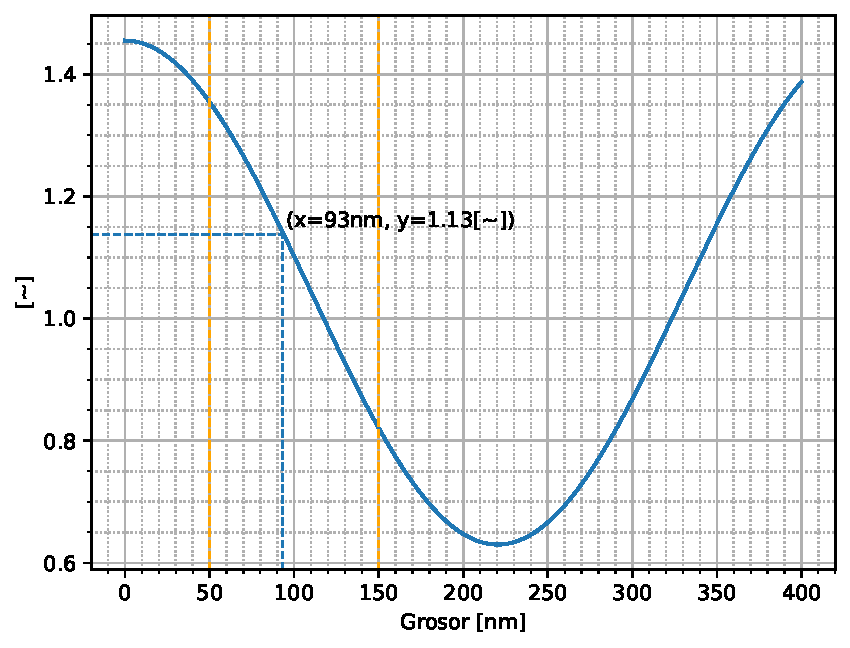
\includegraphics[width=300px]{grosor.pdf}
    \end{center}
    \caption{Resolución gráfica de la equación planteada para encontrar el grosor}
    \label{fig:grosor}
\end{figure}

\newthought{3. Transmitividad del pyrex}

«Compruebe que el valor medido, dentro de las limitaciones de resolución de los aparatos utilizados, resulta con buena aproximación igual al valor teórico para ambas muestras (T=0,917).»

\vspace{5px}

Sea $\vec{E_i}$ una onda plana y uniforme\sidenote{Bajo esta premisa es demostrable que $\vec{P}=\frac{1}{2\eta}|\vec{E}|^2 \, \hat{k}$} incidente y $\vec{E_t}$ la parte transmitida, tenemos

\begin{align}
    \left.
        \begin{aligned}
            \vec{E_i} &= E_{ci} e^{-j\vec{k_i}\cdot\vec{r}} \, \hat{e_t} \quad \\
            \vec{E_t} &= (E_{ci} \tau_t) e^{-j\vec{k_t}\cdot\vec{r}} \, \hat{e_t}
        \end{aligned}
    \right\} \Rightarrow
    \left.
        \begin{aligned}
            |\vec{P_i}| &= \frac{1}{2\eta}|E_{ci}|^2 \quad \\
            |\vec{P_t}| &= \frac{1}{2\eta}|E_{ci}|^2 \, |\tau_t|^2
        \end{aligned}
    \right\}
\end{align}

Donde $\tau_T$ es el resultado de la suma geometrica proveniente de sumar todas las ondas reflejadas.

\begin{align}
    \tau_T = \frac{(1-\rho_{21}^2)\, e^{-jk_2d}}{1-\rho_{21}^2\,e^{-jk_2d}}
\end{align}

El valor de $T$ se define como la relación entre la potencia transmitida y la incidente.

\begin{align}
    T = \frac{|\vec{P_i}|}{|\vec{P_t}|} = |\tau_t|^2
\end{align}

Las $T_{\text{led}}$ y $T_{\text{laser}}$ a partir de las medidas del laboratorio valen $T_{\text{led}}=\frac{\num{0.21}}{\num{0.24}}=\num{0.875}$ y $T_{\text{laser}}=\frac{\num{7.8}}{\num{8.55}}=\num{0.912}$ respectivamente. Se verifica $T_{\text{laser}}\simeq T_{\text{led}}\simeq \num{0.917}$. Además sabemos que $\tau=\pm\sqrt{T}$, por lo que $\tau_{\text{laser}}=\pm\num{0.935}$ y $\tau_{\text{led}}=\pm\num{0.955}$.

\end{document}